% DPF 09 talk on strangeness in nucleon

\documentclass[10pt]{beamer}
\usefonttheme{professionalfonts} % using non standard fonts for beamer
\usefonttheme{serif} % default family is serif
\usepackage{amsmath}
\usepackage{mathtools}
%\documentclass[12pt]{beamerthemeSam.sty}
\usepackage{epsf}
%\usepackage{pstricks}
%\usepackage[orientation=portrait,size=A4]{beamerposter}
\geometry{paperwidth=160mm,paperheight=120mm}
%DT favorite definitions
\def\LL{\left\langle}	% left angle bracket
\def\RR{\right\rangle}	% right angle bracket
\def\LP{\left(}		% left parenthesis
\def\RP{\right)}	% right parenthesis
\def\LB{\left\{}	% left curly bracket
\def\RB{\right\}}	% right curly bracket
\def\PAR#1#2{ {{\partial #1}\over{\partial #2}} }
\def\PARTWO#1#2{ {{\partial^2 #1}\over{\partial #2}^2} }
\def\PARTWOMIX#1#2#3{ {{\partial^2 #1}\over{\partial #2 \partial #3}} }

\def\rightpartial{{\overrightarrow\partial}}
\def\leftpartial{{\overleftarrow\partial}}
\def\diffpartial{\buildrel\leftrightarrow\over\partial}

\def\BI{\begin{itemize}}
\def\EI{\end{itemize}}
\def\BE{\begin{displaymath}}
\def\EE{\end{displaymath}}
\def\BEA{\begin{eqnarray*}}
\def\EEA{\end{eqnarray*}}
\def\BNEA{\begin{eqnarray}}
\def\ENEA{\end{eqnarray}}
\def\EL{\nonumber\\}


\newcommand{\map}[1]{\frame{\frametitle{\textbf{Course map}}
\centerline{\includegraphics[height=0.86\paperheight]{../../map/#1.png}}}}
\newcommand{\wmap}[1]{\frame{\frametitle{\textbf{Course map}}
\centerline{\includegraphics[width=0.96\paperwidth]{../../map/#1.png}}}}

\newcommand{\etal}{{\it et al.}}
\newcommand{\gbeta}{6/g^2}
\newcommand{\la}[1]{\label{#1}}
\newcommand{\ie}{{\em i.e.\ }}
\newcommand{\eg}{{\em e.\,g.\ }}
\newcommand{\cf}{cf.\ }
\newcommand{\etc}{etc.\ }
\newcommand{\atantwo}{{\rm atan2}}
\newcommand{\Tr}{{\rm Tr}}
\newcommand{\dt}{\Delta t}
\newcommand{\op}{{\cal O}}
\newcommand{\msbar}{{\overline{\rm MS}}}
\def\chpt{\raise0.4ex\hbox{$\chi$}PT}
\def\schpt{S\raise0.4ex\hbox{$\chi$}PT}
\def\MeV{{\rm Me\!V}}
\def\GeV{{\rm Ge\!V}}

%AB: my color definitions
%\definecolor{mygarnet}{rgb}{0.445,0.184,0.215}
%\definecolor{mygold}{rgb}{0.848,0.848,0.098}
%\definecolor{myg2g}{rgb}{0.647,0.316,0.157}
\definecolor{abtitlecolor}{rgb}{0.0,0.255,0.494}
\definecolor{absecondarycolor}{rgb}{0.0,0.416,0.804}
\definecolor{abprimarycolor}{rgb}{1.0,0.686,0.0}
\definecolor{Red}           {cmyk}{0,1,1,0}
\definecolor{Grey}           {cmyk}{.7,.7,.7,0}
\definecolor{Lg}           {cmyk}{.4,.4,.4,0}
\definecolor{Blue}          {cmyk}{1,1,0,0}
\definecolor{Green}         {cmyk}{1,0,1,0}
\definecolor{Brown}         {cmyk}{0,0.81,1,0.60}
\definecolor{Black}         {cmyk}{0,0,0,1}

\usetheme{Madrid}


%AB: redefinition of beamer colors
%\setbeamercolor{palette tertiary}{fg=white,bg=mygarnet}
%\setbeamercolor{palette secondary}{fg=white,bg=myg2g}
%\setbeamercolor{palette primary}{fg=black,bg=mygold}
\setbeamercolor{title}{fg=abtitlecolor}
\setbeamercolor{frametitle}{fg=abtitlecolor}
\setbeamercolor{palette tertiary}{fg=white,bg=abtitlecolor}
\setbeamercolor{palette secondary}{fg=white,bg=absecondarycolor}
\setbeamercolor{palette primary}{fg=black,bg=abprimarycolor}
\setbeamercolor{structure}{fg=abtitlecolor}

\setbeamerfont{section in toc}{series=\bfseries}

%AB: remove navigation icons
\beamertemplatenavigationsymbolsempty
\title{
  \textbf {Rotational motion 2}\\
%\centerline{}
%\centering
%\vspace{-0.0in}
%\includegraphics[width=0.3\textwidth]{propvalues_0093.pdf}
%\vspace{-0.3in}\\
%\label{intrograph}
}

\author[W. Freeman] {Physics 211\\Syracuse University, Physics 211 Spring 2015\\Walter Freeman}

\date{\today}

\begin{document}

\frame{\titlepage}

\frame{\frametitle{\textbf{Announcements}}
\BI
\item{Your next homework assignment will be posted tonight or tomorrow, and will be due next Friday}
\item{You will also have a practice exam, posted tonight or tomorrow}
\item{Solutions will be posted next Friday}
\item{Exam 3 will be April 13}
\item{Next Mastering Physics assignment has been posted and is due Tuesday before class} 
\EI
}

\frame{\frametitle{\textbf{Last time: rotational motion}}
  \BI
\item{Most of rotational motion corresponds very directly to linear motion}
\item{Instead of talking about $x$ and $y$, we talk about the angle $\theta$}
\item{Kinematics works the same}
  \pause
\item{{\bf Moment of inertia} $I$ is the rotational analogue of mass}
  \BI
\item{Moment of inertia, like mass, defined with reference to a particular axis}
\item{$I=MR^2$ (if all of the mass in the rotating object is the same distance $R$ from the axis}
\item{$I=\lambda MR^2$ (for more complicated shapes)}
  \EI
  \pause
\item{Rotational kinetic energy is what you'd expect: $KE_{\rm {rot}} = \frac{1}{2}I\omega^2$}
\BI
\item{This is just another form of energy, conserved in the same way and ``alongside'' the things you already learned about}
\item{Work works the same way for rotation as well}
\EI
\pause
\item{The analogue of momentum is {\it angular momentum} $L = I \omega$}
  \BI
\item{This is a different quantity than ordinary momentum, but is also conserved if there are no external torques}
  \EI
  \EI
}

\frame{\frametitle{\textbf{The correspondence table}}
  \centerline{  \begin{tabular}{| c | c |}
      \hline
      Translation & Rotation \\
      \hline
      \hline
      \hline
      Position $x$ & Angle $\theta$ \\
      \hline
      Velocity $v$ & Angular velocity $\omega$ \\
      \hline
      Acceleration $a$ & Angular acceleration $\alpha$ \\
      \hline
      \hline
      $v(t) = v_0 + at$ & $\omega(t) = \omega_0 + \alpha t$ \\
      \hline
      $x(t) = x_0 + v_0 t + \frac{1}{2}at^2$ & $\theta(t) = \theta_0 + \omega_0 t + \frac{1}{2} \alpha t^2$ \\
      \hline
      $v_f^2 - v_0^2 = 2a \Delta x$ & $ \omega_f^2 - \omega_0^2 = 2 \alpha \Delta \theta$ \\
      \hline
      \hline
      Force $\vec F$ & Torque: $\tau=F_\perp r$ \\
      \hline
      Mass $m$ & Moment of Inertia: $I = \lambda MR^2$ \\
      \hline
      \hline
      $\vec F = m \vec a$ & $\tau = I \alpha$ \\
      \hline    
      \hline
      Work = $\vec F \cdot \Delta \vec s$ & Work = $\tau \Delta \theta$ \\
      \hline
      Kinetic energy $\frac{1}{2} mv^2$ & Kinetic energy $\frac{1}{2} I \omega^2$ \\
      \hline
      \hline
      Momentum $\vec p = m \vec v$ & Angular momentum $L = I \omega$ \\
      \hline
  \end{tabular}}
}
  
    \frame{\frametitle{\textbf{Significance of the center of mass}}
      \centerline{\large{We often talk about the center of mass: where is it, and why do we care?}}

        \bigskip
        \bigskip

        \BI
      \item{We know $\vec F = m \vec a$; but what part of the object accelerates?}
        \pause
      \item{Newton's second law gives the acceleration of the {\em center of mass}}
      \BI
    \item{The net force tells you how the center of mass accelerates}
    \item{The net torque tells you the angular acceleration around the center of mass}
    \EI
    \pause
    \bigskip
  \item{For purposes of torque the gravitational force acts at the center of mass}
  \item{For symmetric, uniform objects: the center of mass is at the center!}
  \item{For other objects, it's just a weighted average of all of the parts:}
\EI
\large \bigskip

    \begin{align*}
      x_{\rm {com}} &=& \frac{m_1 x_1 + m_2 x_2 + m_3 x_3 + ...}{m_1 + m_2 + m_3} \\
      \\
      y_{\rm {com}} &=& \frac{m_1 y_1 + m_2 y_2 + m_3 y_3 + ...}{m_1 + m_2 + m_3}
    \end{align*}

  }

    \frame{\frametitle{\textbf{Static equilibrium problems}}
      \large
     \BI
   \item{Often we are presented with a situation where nothing moves, and we have to solve for something}
   \item{No acceleration of the center of mass: $\sum \vec F = 0$}
   \item{No angular acceleration: $\sum \tau = 0$ about {\it any} pivot point}
   \item{Can generate enough equations this way to solve for all unknowns}
     \pause
   \item{Strategy: choose the pivot to be aligned with a force you don't know and don't care about}
     \EI
   }

   \frame{\frametitle{\textbf{A sample problem: forces on a bar}}
     \Large
     A bar is suspended by a hinge at one end, and by a cable at the other making an angle $\theta$ with the vertical.
     If the bar has mass $m$, what is the tension in the cable?
   
     \bigskip
     
     (Illustrated with demo equipment; solution on document camera)

     \pause

     \bigskip
     \bigskip


     What is the (vector) force at the hinge?
 }


\frame{\frametitle{\textbf{One more thing: another way of computing torque}}
  \centerline{\large Last time we saw that the torque $\tau = F_\perp r$}
  \bigskip
  \centerline{\large ... but there's another way to compute it which is sometimes more helpful}
  \bigskip
  \BI
\item{Note that $F_\perp = F\, \sin\,\theta$, so $\tau = F r \, \sin \theta$}
\item{We can think of the torque in any other equivalent way; there is another one that's often useful}
\item{The way I taught you yesterday: {\bf ``The radius vector, times the component of force perpendicular to it''}}
\item{The alternative: {\bf ``The force vector, times the component of the radius perpendicular to it''}}
\EI
\centerline{\large{Here's the figure from the text:}}
\centerline{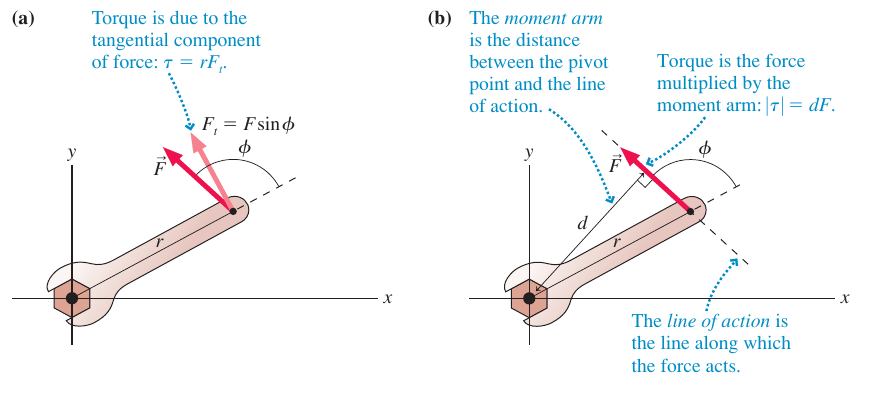
\includegraphics[width=0.6\textwidth]{momentarm.png}}
\bigskip
\centerline{I'll draw a clearer version on the document camera}
}

\frame{\frametitle{\textbf{One more thing: another way of computing torque}}
  \centerline{\large Last time we saw that the torque $\tau = F_\perp r$}
  \bigskip
  \centerline{\large ... but there's another way to compute it which is sometimes more helpful}
  \bigskip
  \BI
\item{Note that $F_\perp = F\, \sin\,\theta$, so $\tau = F r \, \sin \theta$}
\item{We can think of the torque in any other equivalent way; there is another one that's often useful}
\item{The way I taught you yesterday: {\bf ``The radius vector, times the component of force perpendicular to it''}}
\item{The alternative: {\bf ``The force vector, times the component of the radius perpendicular to it''}}
\EI
\bigskip
  \centerline{\Huge{$\tau = F_\perp r = F r_\perp = F r \, \sin \theta$}}
  \bigskip
  \bigskip
  \centerline{(where $\theta$ is the angle between the radius and force vectors)}

  \pause

  \centerline{NB: Your book calls $r_\perp$ the ``moment arm''}
  }

  \frame{\frametitle{\textbf{A sample problem: distribution of weight in a truck}}
    \large
    A 2000 kg rear wheel drive pickup truck has a wheelbase 5 meters long. 
    Its center of mass is located 150 cm behind the front wheels, and 130 cm above the ground. 
    What is the fastest it can accelerate, if $\mu_s = 0.6$?

    \pause
    
    \bigskip
    \bigskip

    The limiting factor is the traction force: static friction on the rear wheels.

    \pause

    \bigskip
    \bigskip

    Compute torque about the front wheels: 

    \begin{align*}
      1.5mg &= 5 F_{N,{\rm rear}} \\
      F_{N,{\rm rear}} &= 0.3 mg \\
      F_{f,{\rm max}} &= \mu_s F_{N,{\rm rear}} =0.18 mg \\
      a_{\rm {max}} &= 0.18 g
    \end{align*}
    
  }





  \frame{\frametitle{\textbf{A few nifty demos on angular momentum}}
      \large
      \centerline{Angular momentum $L = \sum I \omega$ is conserved in the absence of external torques}
      \BI
      \pause
    \item{Dumbbell demo: if $I$ goes down, $\omega$ goes up}
      \pause
    \item{Bike wheel demo: $\sum L = {\rm constant}...$}
      \pause
  \item{We learned about rotation in 2D, where $\omega$, $L$, and $\tau$ are scalars}
  \item{In 3D they're vectors, and the behavior can be downright weird!}
    \EI
    }

    \frame{\frametitle{\textbf{Finding the balancing point}}
      \Large
      A bar of mass 5 kg and length 1 m has a weight of mass 1 kg resting on one end. At what point must it be supported
      if it is to balance?
\normalsize
      \pause
      \bigskip
      \bigskip
      \bigskip
      \bigskip

      Strategy: 
      \BI
    \item{Draw a ``number line'' by your force diagram and label coordinates}
    \item{Introduce a variable corresponding to the thing you're trying to find}
      \EI
    }

    \frame{\frametitle{\textbf{Finding the balancing point}}
      \Large
      A bar of mass 5 kg and length 1 m has a weight of mass 1 kg resting on one end. At what point must it be supported
      if it is to balance?
\normalsize
      \pause
      \bigskip
      \bigskip
      \bigskip
      \bigskip

      Strategy: 
      \BI
    \item{Draw a ``number line'' by your force diagram and label coordinates}
    \item{Introduce a variable corresponding to the thing you're trying to find}
    \item{Can compute torques about {\it any} pivot; which is easiest?}

      \EI
    }
    
       \frame{\frametitle{\textbf{Finding the balancing point}}
      \Large
      A bar of mass $m$ and length $L$ has a weight of mass $M$ resting on one end. At what point must it be supported
      if it is to balance?
\normalsize
      \pause
      \bigskip
      \bigskip
      \bigskip
      \bigskip

      Same method as before, but note:
      \BI
    \item{The point of support is also the center of mass}
    \item{The converse is also true: an object's center of mass must be within its base of support if it is to stay put}
      
      \EI
    }
 
    \end{document}
